\section{Metode Garbage Collection Lanjutan}

Setelah memahami mekanisme dasar \textit{Reference Counting} dan \textit{Mark-and-Sweep}, kompilator modern sering menggunakan teknik tambahan untuk menangani fragmentasi dan meningkatkan performa.

\subsection{1. Mark-Compact Garbage Collection}
Kelemahan \textit{Mark-and-Sweep} murni adalah ia meninggalkan "lubang" (\textit{holes}) di seluruh heap. \compiler{Mark-Compact} menyelesaikan ini dalam tiga fase:
\begin{enumerate}
    \item \textbf{Mark}: Menandai semua objek yang masih bisa dijangkau (\textit{reachable}) dari \textit{GC Roots} (Stack, Register, Variabel Global).
    \item \textbf{Compact}: Memindahkan semua objek yang ditandai ke satu sisi heap, sehingga semua memori kosong terkumpul menjadi satu blok besar yang kontinu.
    \item \textbf{Update}: Memperbarui semua pointer di program agar merujuk ke lokasi baru objek yang telah dipindah.
\end{enumerate}

\subsection{2. Copying Garbage Collection (Semi-space)}
Algoritma ini membagi heap menjadi dua bagian berukuran sama: \textbf{From-Space} dan \textbf{To-Space}.
\begin{enumerate}
    \item Alokasi hanya dilakukan di \textit{From-Space}.
    \item Saat penuh, GC menyalin hanya objek yang \textit{live} ke \textit{To-Space} secara berurutan (kontinu).
    \item Seluruh isi \textit{From-Space} yang tersisa (sampah) langsung dibuang secara massal.
    \item Peran \textit{From-Space} dan \textit{To-Space} ditukar untuk siklus berikutnya.
\end{enumerate}
\textbf{Keuntungan}: Alokasi menjadi sangat cepat (cukup menaikkan pointer \textit{top of heap}) dan fragmentasi otomatis hilang. \textbf{Kerugian}: Membutuhkan kapasitas memori dua kali lipat dari yang sebenarnya bisa digunakan.

\begin{figure}[!htbp]
    \centering
    \adjustbox{max width=0.8\textwidth,center}{%
    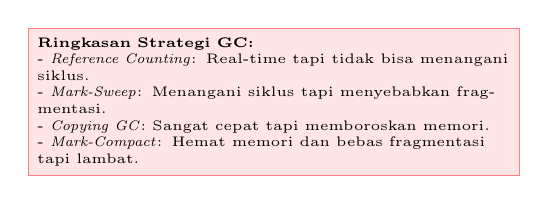
\begin{tikzpicture}[
        rect/.style={rectangle, draw=red!50, fill=red!10, text width=6cm, font=\tiny}
    ]
    \node[rect] (gc) {
        \textbf{Ringkasan Strategi GC:}\\
        - \textit{Reference Counting}: Real-time tapi tidak bisa menangani siklus.\\
        - \textit{Mark-Sweep}: Menangani siklus tapi menyebabkan fragmentasi.\\
        - \textit{Copying GC}: Sangat cepat tapi memboroskan memori.\\
        - \textit{Mark-Compact}: Hemat memori dan bebas fragmentasi tapi lambat.
    };
    \end{tikzpicture}%
    }
    \caption{Perbandingan Algoritma Manajemen Memori Otomatis}
\end{figure}
